\documentclass[aps,prb,reprint,noeprint,superscriptaddress]{revtex4-1}
\pdfoutput=1
\usepackage[utf8]{inputenc}
\usepackage[english]{babel}
\usepackage{microtype}
\usepackage{amsmath,amssymb,amsfonts}
\usepackage{braket}
\usepackage{bm}
\usepackage{graphicx}
\usepackage{booktabs}
\usepackage{comment}
\usepackage{siunitx}
\usepackage{float}
\usepackage[
    pdftitle={},
    pdfauthor={},
    colorlinks=true,
    unicode=true,
    pdfborder={0 0 0},
    allcolors=blue
]{hyperref}

\renewcommand{\vec}[1]{\bm{#1}}
\newcommand{\im}{\mathrm{i}}
\newcommand{\e}{\mathrm{e}}
\renewcommand{\Im}{\operatorname{\mathsf{Im}}}
\renewcommand{\Re}{\operatorname{\mathsf{Re}}}
\newcommand{\vk}{{\vec k}}
\newcommand{\vq}{{\vec q}}
\newcommand{\VV}[2]{\begin{pmatrix}#1\\#2\end{pmatrix}}
\newcommand{\VVT}[2]{\begin{pmatrix}#1 & #2\end{pmatrix}}
\newcommand{\VVV}[3]{\begin{pmatrix}#1\\#2\\#3\end{pmatrix}}
\newcommand{\VVVT}[3]{\begin{pmatrix}#1 & #2 & #3\end{pmatrix}}
\newcommand{\MM}[4]{\begin{pmatrix}#1 & #2 \\ #3 & #4\end{pmatrix}}

\begin{document}

\title{Time-resolved optical conductivity and Higgs oscillations\\in two-band dirty superconductors}

\author{Rafael Haenel}
\affiliation{Max Planck Institute for Solid State Research,
70569 Stuttgart, Germany}
\affiliation{Quantum Matter Institute, University of British Columbia, Vancouver V6T 1Z4, Canada}

\author{Paul Froese}
\affiliation{Max Planck Institute for Solid State Research,
70569 Stuttgart, Germany}
\affiliation{Quantum Matter Institute, University of British Columbia, Vancouver V6T 1Z4, Canada}


\author{Dirk Manske}
\affiliation{Max Planck Institute for Solid State Research,
70569 Stuttgart, Germany}

\author{Lukas Schwarz}
\affiliation{Max Planck Institute for Solid State Research,
70569 Stuttgart, Germany}


\date{\today}

%%%%%%%%%%%%%%%%%%%%%%%%%%%%%%%%%%%%%%%%%%%%%%%%%%%%%%%%
\begin{abstract}
...
\end{abstract}
%%%%%%%%%%%%%%%%%%%%%%%%%%%%%%%%%%%%%%%%%%%%%%%%%%%%%%%%




\maketitle


%%%%%%%%%%%%%%%%%%%%%%%%%%%%%%%%%%%%%%%%%%%%%%%%%%%%%%%%
\section{Introduction}
\label{sec:introduction}
%%%%%%%%%%%%%%%%%%%%%%%%%%%%%%%%%%%%%%%%%%%%%%%%%%%%%%%%

When a global symmetry is spontaneously broken, collective excitations emerge.
In the case of a superconductor, where the local order parameter $\Delta
e^{i\varphi}$ acquires a
finite value below a critical temperature $T_C$, two bosonic modes appear: the
massive Higgs mode and a massless Goldstone mode. They may be seen as
longitudinal and phase fluctuations of the complex order parameter in a Mexican
hat free energy. In the presence of Coulomb interaction, the Goldstone mode is
shifted to optical frequencies
by means of the Anderson Higgs mechanism while the Higgs mode remains
a stable gapped excitation in the Terahertz regime.

In a two-band superconductor, two gapless Higgs modes and two phase modes exist.
While the global phase fluctuations occur only at energies close to the plasma
frequency, relative phase fluctuations, termed Leggett mode, 
persist as a gapped excitation at low energies.

Experimental observation of Higgs and Leggett collective modes is difficult.
Since the
Higgs field is a scalar quantity, no linear coupling to the vectorial
electromagnetic field can exist. Thus, there are no direct experimental signatures in
linear response and experiments need to be performed in the non-linear
regime. Here, the challenge is twofold: intense light sources are required
but experiments also have to be performed on energy scales mostly
within the superconducting gap such that optical excitation of quasiparticles does not deplete 
the condensate. 

Recent developments in ultrafast Terahertz spectroscopy have caused 
a surge in interest in collective excitations in superconductors and
experimental signatures of the Higgs mode have now been observed in various
materials.

Experiments performed so far consist of two approaches. First, samples are
illuminated in a pump-probe setup where
an excitation of the Higgs mode by a single-cycle THz pump appears as an oscillation of the
probe signal as a function of pump-probe delay. In a second type of experiments, 
the Higgs mode is resonantly driven
by an intense multi-cycle pulse that yields a electrical field
component of three times the pump frequency in the reflected or transmitted
beam. Theoretically, time-resolved oscillation of the gap in angle-resolved
photoemission (ARPES) spectra has also been studied as a third characterization
scheme. Additionally, Higgs excitation has been proposed as
its own spectroscopic method based on the insight that the gap symmetry of a
superconductor can be classified from measurements of the condensate
oscillations in different geometries.

The fact that characteristics of the Higgs boson in superconductors are
observable in experiments at all was not obvious from the beginning. Initially
theoretical calculations in the clean limit predicted extremely weak
experimental signatures unobservable with even today's experimental equipment.
Only recently the role of impurities has been appreciated in achieving more
realistic theoretical predictions. [list publications: Silaev, Murotani,
Benfatto] In the clean limit, the Higgs mode only
diamagnetically couples to the gauge field. Presence of impurities additionally enables
a paramagnetic coupling which becomes the dominant contribution even for small disorder. 
It was
further shown that impurity scattering yields qualitatively different behavior
in the polarization dependence of the pump pulses.

An outstanding question MgB2. Murotani. Demler experiment.


[How does this paper go beyond the work of Murotani and Shimano?]
\begin{itemize}
  \item time resolved optical conductivity
  \item discussion of the second gap of MgB2 - why can't we see it in
    optical experiment?
  \item Third harmonic generation where pulse frequency is swept. (todo: also
      sweep the temperature, show decomposition in terms of QP, Higgs, Legget
    mode)
  \item (Discussion of four cases)
  \item Coupling of Higgs and Leggett mode. Do they actually couple?
  \item Presentation using SI units to make everything easily comparable to
    experiments.
  \item Discussion of the paramagnetic activation in terms of diagrams?
\end{itemize}

This article is organized as follows. In Sec. \ref{sec:model} we briefly review
key aspects of the model as introduced by Murotani and Shimano []. We then
discuss the case of a single-band superconductor in a pump-probe scenario
in Sec. \ref{sec:singleband} and make reference to available experimental data. 
In Sec. \ref{sec:multiband} we study in detail the case of a two-band
superconductor motivated by material parameters of MgB$_2$ with different 
impurity concentrations of the conduction bands. We summarize all results in
Sec. \ref{sec:conclusion}.







%%%%%%%%%%%%%%%%%%%%%%%%%%%%%%%%%%%%%%%%%%%%%%%%%%%%%%%%
\section{Model}
\label{sec:model}
\subsection{Hamiltonian}
%%%%%%%%%%%%%%%%%%%%%%%%%%%%%%%%%%%%%%%%%%%%%%%%%%%%%%%%
We consider a meanfield description of a multiband $s$-wave BCS superconductor,

\begin{eqnarray}
  \mathcal{H}_{0} = \sum_{i\mathbf{k}\sigma}  
	\varepsilon_{i\mathbf{k}}c_{i\mathbf{k}\sigma}^\dagger
	c_{i\mathbf{k}\sigma} + \sum_{i\mathbf{k}}^{}
	\left( \Delta_i c_{i\mathbf{-k}\uparrow }^\dagger
	c_{i\mathbf{k}\downarrow }^\dagger  \right) \,,
\end{eqnarray}

where $\varepsilon_{i\mathbf{k}} = s_i \left(\mathbf{k}^2/2m_i -
\varepsilon_{F_i}\right)$ is the parabolic dispersion of the $i$-th band with
Fermi-energy $\varepsilon_{F_i}$ and electron mass $m_i$. 
$s_i=\pm$ determines electron/hole-like character of the respective band. The intraband 
order parameter is self-consistently determined by the BCS equation
$\Delta_i = \sum_{j\mathbf{k}}^{}U_{ij} \langle c_{j-\mathbf{k}\downarrow
}c_{j\mathbf{k}\uparrow }\rangle$. Interband pairing in BCS superconductors is
considered weak (discussion, reference) and has been neglected in our model. 

Order parameters of different bands are mixed by off-diagonal terms of the
coupling matrix $U_{ij}$. In the present work, we parametrize
gap-mixing by a parameter $v$ and define
\begin{eqnarray*}
  U_{ij} = 
  \begin{pmatrix}
    U_{11} & v U_{11} \\
    v U_{11} & U_{22}
  \end{pmatrix}
\end{eqnarray*}
in the case of a two-band superconductor.
For given $\Delta_i$ and $v$ we can thus find $U_{11}$ and
$U_{22}$ such that the gap equation is satisfied.

To model an experimental probe with a laser pulse, we introduce a time dependent gauge vector
potential $\mathbf{A}(t)=\mathbf{e} A(t)$ by means of minimal coupling,
\begin{eqnarray*}
	\mathcal{H}_{1} = -\sum_{i\mathbf{kk'}\sigma}^{}
	\mathbf{J}_{i\mathbf{kk'}} \cdot \mathbf{A} \,
	c_{i\mathbf{k}\sigma}^\dagger  c_{i\mathbf{k}'\sigma} +
	\sum_{i\mathbf{k}\sigma}^{} \frac{s_i e^2}{2m_i} \mathbf{A}^2 \,
	c_{i\mathbf{k}\sigma}^\dagger c_{i\mathbf{k}\sigma}\,.
\end{eqnarray*}
$J_{i\mathbf{kk'}}=\bra{i\mathbf{k}}\frac{e\mathbf{p}_i}{m_i}
\ket{i\mathbf{k'}}$ are intraband transition matrix elements of the current
operator. (Discussion why we neglect interband transitions). The two terms in
$\mathcal{H}_1$ corresponds to the paramagnetic and diamagnetc coupling to the laser field,
respectively.
The full Hamiltonian is given by $\mathcal{H} = \mathcal{H}_{0} + \mathcal{H}_{1}$.

\subsection{Impurity scattering}
\label{sec:MB}
In a clean system momentum conservation yields $\mathbf{J}_{i\mathbf{kk'}} \sim
\delta_{\mathbf{kk'}}$, or $\mathbf{J}_{i\mathbf{kk'}} \sim
\delta_{\mathbf{k,k'}\pm\mathbf{q}}$ if a photon wavevector $\mathbf{q}$ is
considered. In disordered systems translational invariance is broken, so that
transitions between states of different momentum are allowed. Here, we adopt the
approach of Murotani and Shimano [] and model the effects of impurities by
means of the Mattis-Bardeen (MB) substitution []. It relies on approximating the
transition matrix elements $J_{i\mathbf{kk'}}$ as a
Lorentzian in momentum transfer space, explicitly written as
\begin{eqnarray}
	\langle \left|\mathbf{e} \cdot
	\mathbf{J}_{i\mathbf{kk'}}\right|^2\rangle_{\text{Av}}
	&=& \int \frac{d\Omega_\mathbf{k}}{4\pi} \frac{d\Omega_\mathbf{k}'}{4\pi}
	\left|\mathbf{e} \cdot \mathbf{J}_{i\mathbf{kk'}}\right|^2
	\\
	&\approx& \frac{(e v_{F_i})^2}{3 \pi N_i(0)} 
	\frac{\gamma_i}{\left(\varepsilon_{i|\mathbf{k}|}-\varepsilon_{i|\mathbf{k}'|}\right)^2
	+ \gamma_i^2} \,,
	\label{eq:MB}
\end{eqnarray}
with Fermi velocity $v_{F_i}$ density of states of the Fermi level $N_i(0)$ and
impurity scattering rate $\gamma_i$. Note that we are considering an effectively
one-dimensional quantity
where all angular degrees of freedom have been averaged out.
Physically, this means that impurity scattering occurs with equal probability
between all states within a shell around the Fermi sphere.
A derivation of this matrix element
following [Murotani] is reviewed in Appendix \ref{apdx:MB}.

An optical transition can be resonantly driven only if (1) an energy matching
condition and (2) a momentum 
matching condition is satisfied. Assuming a transition energy of $\Delta$,
condition
(1) can be satisfied by tuning the optical pulse frequency to $\omega=\Delta$.
Let us for simplicity consider a one-dimensional system. If
$\Delta$ is sufficiently small, the parabolic dispersion can be linearized at
the Fermi level, $\varepsilon_k = v_F k$. Then, a momentum of $\Delta/v_F$ 
is necessary to satisfy condition (2). In a clean system it then follows that
photoexcitation within a single band is not possible
if bandfolding effects are also neglected.
In a weakly disordered system, momentum is no longer a good quantum
number. Here, momentum broadening $\delta k$ can be viewed as providing the necessary
momentum and the transition becomes resonant for $v_F \delta k=\Delta$. For
strong disorder the concept of momentum is lost and any two states
can be connected by satisfying condition (1) only.

In the MB approximation, $\mathbf{k}$ is still treated as an exact quantum
number of the unperturbed system but presence of impurities 
broadens momentum conservation of the transition matrix element
$\mathbf{J}_{i\mathbf{kk'}}$ into a Lorentzian momentum transfer distribution of
width $\gamma_i$ centered at zero momentum transfer. 
It is straightforward to check that for an excitation of energy $\Delta$ 
the matrix element gives the largest contribution 
for an impurity scattering rate of $\gamma_i=\Delta$. 

One may picture the Higgs excitation as a two-photon excitation process, where
the first photon populates a virtual intermediate state at energy $\Delta$ above
the groundstate and the second photon contributes the remaining $\Delta$ to
establish resonance with the Higgs mode at $2\Delta$.
Based on
these arguments, we can expect the largest enhancement of the Higgs resonance at 
$\gamma_i = \Delta_i$.

[Discussion of relevant scales $\Delta, \gamma, \omega_D, \varepsilon_F$.
Specifically, what happens when $\gamma>\omega_D$??]


\subsection{Equations of motion}

We solve for the time dynamics of above Hamiltonian using a density matrix
approach. To this end, we define the density matrix $\rho =
\ket{\psi_0}\bra{\psi_0}$, or, in the basis of single-particle/hole excitations,
$\mathcal{B}=\left\{ c_{i\mathbf{k}\uparrow }\ket{0},\, c_{i-\mathbf{k}\downarrow
}\ket{0} \right\}$
\begin{eqnarray*}
  \rho = 
  \begin{pmatrix}
    \rho_{i\mathbf{kk'}}^{11} &
    \rho_{i\mathbf{kk'}}^{12} \\
    \rho_{i\mathbf{kk'}}^{21} &
    \rho_{i\mathbf{kk'}}^{22}
  \end{pmatrix}
  =
  \begin{pmatrix}
    \langle c_{i\mathbf{k}\uparrow }^\dagger c_{i\mathbf{k}'\uparrow }\rangle
    &
    \langle c_{i\mathbf{k}\uparrow }^\dagger c_{i-\mathbf{k}'\downarrow
    }^\dagger \rangle
    \\
    \langle 
    c_{i-\mathbf{k}\downarrow }c_{i\mathbf{k'}\uparrow }
    \rangle
    &
    \langle 
    c_{i-\mathbf{k}\downarrow }c_{i\mathbf{-k'}\downarrow }^\dagger 
    \rangle
  \end{pmatrix}
\end{eqnarray*}

The time dependence of $\rho$ is given by the Heisenberg equation of motion,
\begin{eqnarray*}
  i\partial_t \rho = \left[ \rho, H \right]
\end{eqnarray*}
where $H$ is the operator $\mathcal{H}$ in the basis $\mathcal{B}$. 

We are interested in computing the dynamics of the current
$ \mathbf{j} = -\big\langle \frac{\delta \mathcal{H}}{\delta
\mathbf{A}}\big\rangle =
\mathbf{j}_P + \mathbf{j}_D$, consisting of a paramagnetic and diamagnetic
contribution,
\begin{eqnarray*}
  \mathbf{j}_P 
	&=&
  	\sum_{i\mathbf{kk'}}^{}
	\mathbf{J}_{i\mathbf{kk'}}\,
	\left( 
	  \rho_{i\mathbf{kk'}}^{11}
	  -\rho_{i\mathbf{kk'}}^{22}
	  +1
	\right)
	\\
  \mathbf{j}_D &=& -\sum_{i\mathbf{k}\sigma}^{} \frac{s_i e^2}{2m_i} 
  \mathbf{A} \,
	\left( 
	  \rho_{i\mathbf{kk}}^{11}
	  -\rho_{i\mathbf{kk}}^{22}
	  +1
	\right)
\end{eqnarray*}
and we compute the dynamics of the superconducting order parameter
\begin{eqnarray*}
  \Delta_i = \sum_{j\mathbf{k}}^{}U_{ij} 
  \rho_{j\mathbf{kk}}^{21} \,.
\end{eqnarray*}
To apply the MB substitution we further expand above equation of motions in
orders of $A(t)$. To account for effects of a THG response, we consider terms up to
third order. As detailed in Appendix \ref{apdx:model}, the current only has odd order
components $\mathbf{j} = \mathbf{j}\big|_0 +\mathbf{j}\big|_3 + \dots$ and the
gap only contains even contributions of $A$, $\Delta = \Delta\big|_0 +
\Delta\big|_2 +\dots$. 

Finally, we exploit the rotational invariance of our model and perform the
integral over angular degrees of freedom explicitly. Thus, by replacing all momentum summations
by an integral 
$\sum_{\mathbf{k}}^{} \rightarrow
N_i(0)\int_{}^{}d\varepsilon_{i\mathbf{k}}\int_{}^{}
\frac{d\Omega_{\mathbf{k}}}{4\pi}$, we effectively reduce the model to a
one-dimensional system. Note that rotational invariance of our continuum model
neglects polarization dependence of observable quantities.


We are left to compute the equations of motion of the
angle-averaged quantities
\begin{eqnarray*}
  R^{1/3,n}_{\varepsilon_{|\mathbf{k}|}} &=& 
  \int_{}^{}\frac{d\Omega_{\mathbf{k}}}{4\pi}
  \int_{}^{}\frac{d\Omega_{\mathbf{k'}}}{4\pi}
  \mathbf{J}_{i\mathbf{kk'}} \, \rho_{i\mathbf{kk'}}^{nn}\big|_{1/3}
  \\
  r^{nm}_{\varepsilon_{|\mathbf{k}|}} &=& 
  \int_{}^{}\frac{d\Omega_{\mathbf{k}}}{4\pi}
  \rho_{i\mathbf{kk}}^{nm}\big|_{2} \,.
\end{eqnarray*}
We solve them numerically using a [Runge-Kutta] solver on a discretized energy grid
$\varepsilon_{|\mathbf{k}_i|}$ of up to $10^3$ points in the interval $\left[
  -\omega_D, \omega_D
\right]$ (why do we use $\omega_D$???).
A detailed derivation and an explicit presentation of the full equations of
motion is given in Appendix \ref{apdx:model}.









\section{Single-band superconductivity}

\begin{figure}[ht]
	\centering
	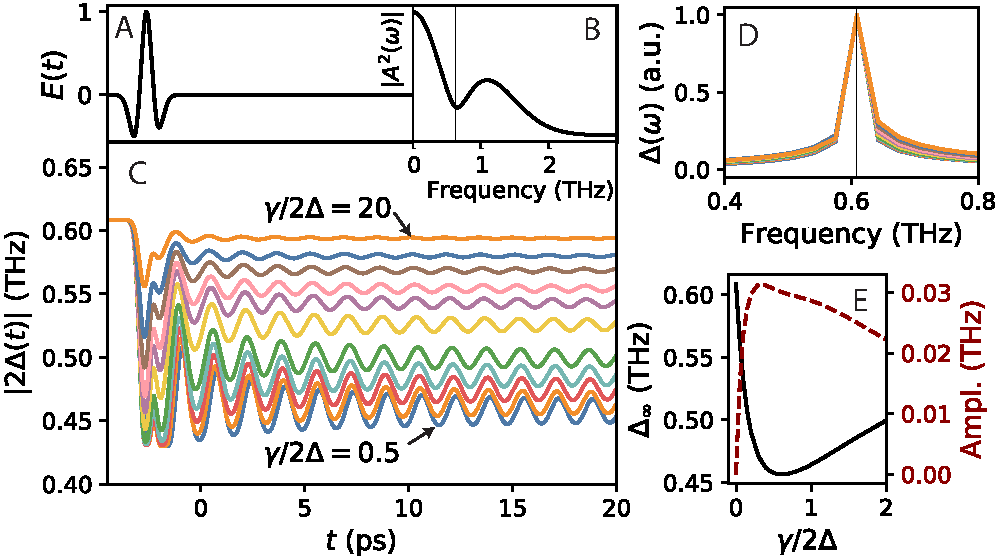
\includegraphics[width=\columnwidth]{figures/fig1.pdf}
	\caption{(a) Pulse field $E(t)$ realizing a quench. (b) Spectral
	composition $|A(\omega)|$. The gray shaded area illustrates the
quasi-particle continuum. (c) Spectral compositon $A^2(\omega)$ of the second
order component $A^2(t)$ responsible for excitation of collective modes. The
peak around zero frequency corresponds to a DFG process while the peak at finite
$\SI{1.2}{\tera\hertz}$ is a SFC process. (c) Evolution of the magnitude of the
order parameter $\left|2\Delta(t)\right|$ for impuritiy strength varying from
$\gamma/2\Delta=0.5$ to $20$ and Fourier spectrum of the gap oscillations (d).
(e) Relaxation value $\Delta_{\infty}$ and amplitude of oscillation show a very
similar dependence as a function of disorder strength which has maximum effect
at around $\gamma \approx \Delta$.}
\label{fig:singleband-gap}
\end{figure}
\label{sec:singleband}

Motivated by the experiment of Matsunaga et al. [] we choose parameters
$\Delta_{\text{eq}}=\SI{1.3}{\milli\electronvolt}$,
$\varepsilon_{F}=\SI{1}{\electronvolt}$, $m=0.78 m_e$, $s=1$ that reflect
measurements and ab-initio calculations on NbN [DFT-reference].
The Debye energy for NbN is order order of 
$\omega_D = \SI{50}{\milli\electronvolt}$, but
for better numerical resolvability we choose $\omega_D =
\SI{20}{\milli\electronvolt}$.

We choose the electromagnetic pulse form $A(t) = A_0 \exp\left( -(t-t')^2/2\tau^2
\right)\cos \Omega t$ and choose coefficients to match the reported data 
of [Matsunaga]. The resulting
electrical field waveform is shown in Fig. \ref{fig:singleband-gap}(a). 

A characteristic property of a pump pulse is its pulse 
length $\tau$ compared to the natural
timescale of the superconductor, $1/\Delta$. For $\tau \ll \hbar / \Delta$
the superconductor is \textit{quenched}, while it is \textit{adiabatically
driven} in the
opposite limit of $\tau \gg  1 / \Delta$. 
The different behavior in the two limits can be intuitively understood 
from the simple relation
\begin{eqnarray*}
  \delta \Delta(\omega) \sim K(\omega) A^2(\omega)
\end{eqnarray*}
where $K(\omega)$ is the optical nonlinear kernel []. Presence of a collective mode
translates into a peak of the optical Kernel at the characteristic mode energy
$\omega=2\Delta$, illustrated in Fig. \ref{fig:singleband-gap}(c) by a vertical
line.
$A^2(\omega)$  
is the Fourier transform of the squared vector
potential $A(t)^2$ and hence given by a self-convolution of $A(\omega)$. $A^2(\omega)$, shown in Fig. 
\ref{fig:singleband-gap}(c), has a double-peaked structure. The first peak,
centered at $\omega=0$, corresponds to a difference frequency process (DFG),
while the second peak at $\omega=2\Omega$ corresponds to a sum frequency process
(SFG). For $\Delta\tau\ll 1$, the frequency structure of $A^2(\omega)$ is very
broad. The response of $\delta\Delta(\omega)$ is then dominated by the sharp
resonance peak of $K(\omega)$ giving rise to pronounced $2\Delta$-oscillations
of the superconducting gap in the time domain. 
Since the DFG peak is 
guaranteed to overlap with the Higgs resonance,
these oscillations will always be present,
independent of the frequency of the optical pulse. The SFG process only contributes
if the pulse frequency lies in the vicinity of $\Omega \approx \Delta$.

In the transient limit, $\Delta \tau\gg 1$, the frequency structure of
$\delta\Delta(\omega)$ is dominated by the sharp SFG peak of the pulse. The gap
will show a forced oscillation with frequency $2\Omega$ which, however, is
resonantly enhanced when $2\Omega\approx2\Delta$.

Following Matsunaga, we choose a pulse with $\Delta \tau = 0.x$, closest to the
quench scenario. The superconducting order parameter indeed shows characteristic
oscillations with frequency $2\Delta=\SI{6.x}{\tera\hertz}$ as shown in Figs.
\ref{fig:singleband-gap}(d-e). The gap can be seen to respond to the THz pulse
by a marked drop followed by damped oscillations around a new value
$\Delta_{\infty}$. [$\left|\Delta^{eq}-\Delta_{\infty}\right| \propto
  \int_{}^{}d\omega \sigma'(\omega) A(\omega).$, 
Discussion why it does not oscillate with $\Delta_{\infty}$] 

Both the oscillation amplitude and $\Delta_{\infty}$ show a
strong dependence on the impurity scattering rate peaked at $\gamma\approx
\Delta^{eq}$, see Fig. \ref{fig:singleband-gap}(f). For $\gamma\rightarrow 0$
the Higgs resonance vanishes. [Discussion photon $\mathbf{q}$ and $A^2$ term] These results underline the
importance of impurity scattering for the excitation efficiency of collective
Higgs modes uncovered recently [].
We can understand this result by examining the matrix elements of the current
operator, Eq. (\ref{eq:MB}), following the discussion of Sec. \ref{sec:MB}.
Indeed, the $\gamma$-dependence closely follows
the functional form $\gamma/(\Delta_{eq}^2+\gamma^2)$.


\begin{figure}[t]
	\centering
	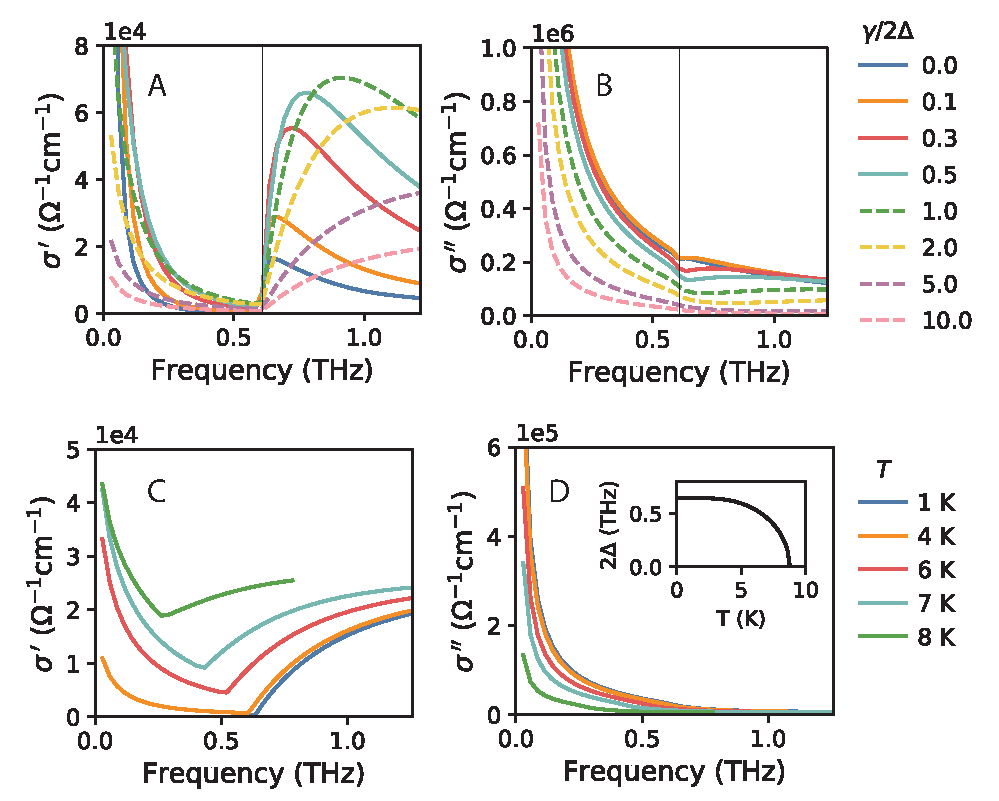
\includegraphics[width=\columnwidth]{figures/fig2.pdf}
	\caption{Real part $\sigma'$ (A,C) and imaginary part $\sigma''$ (B,D)
		of optical conductivities to first order in $A$ 
	for various impurity scattering rates at $T=\SI{4}{\kelvin}$ (A,B) and
various temperatures at $\gamma/2\Delta=10$. $\sigma'$ show a characteristic
conductivity gap below $T_C$ and both $\sigma'$, $\sigma''$ diverge in the
static limit.}
\label{fig:cond-lin}
\end{figure}

\begin{figure}[t]
	\centering
	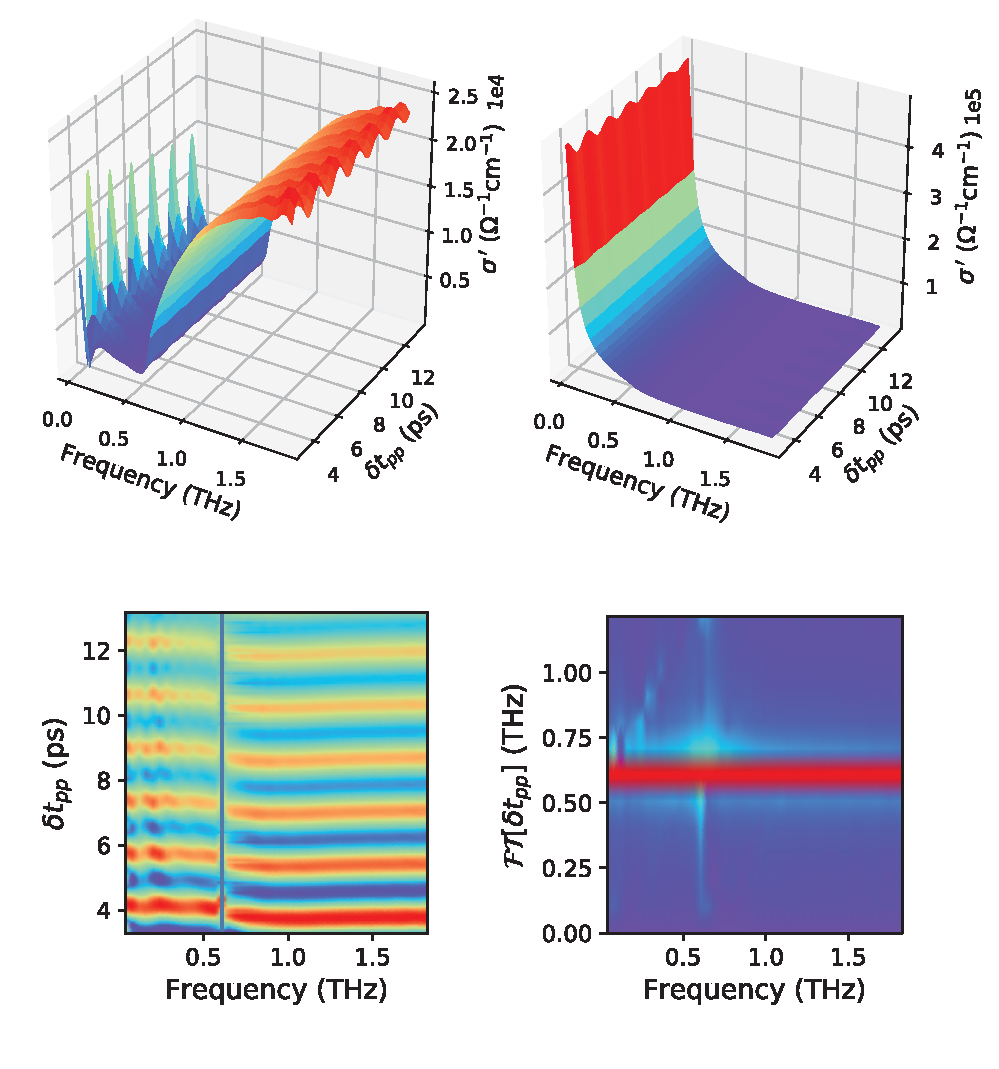
\includegraphics[width=\columnwidth]{figures/fig3.pdf}
	\caption{(A,B) Conductivity spectra for sweeped pump-probe delay $\delta
	t_{\text{p-p}}$ to third order in $A$. (C) False-color plot of
$\sigma' $ which was average-subtracted and normalized to show the oscillations.
A phase shift occurs across the resonance at $2\Delta_{\text{eq}}$ of the quench pulse
frequency. (D) Fourier spectrum of panel (C) showing that frequency of
conductivity oscillation is peaked at $2\Delta_{\text{eq}}$.}
\label{fig:cond-pp}
\end{figure}

Next we compute the optical conductivity in linear response
\begin{eqnarray*}
  \sigma_0(\omega)\big=\frac{j(\omega)\big|_1}{i\omega A(\omega)} \,.
\end{eqnarray*}
Real and
imaginary parts $\sigma'(\omega),\sigma''(\omega)$ are plotted 
in Fig. \ref{fig:cond-lin}(a-b) for various impurity
concentrations and in Fig. \ref{fig:cond-lin} for various temperatures.
At low temperatures $\sigma'$ shows a clear conductivity gap below $2\Delta^{eq}$. 
In the clean limit, a pronounced coherence peak is observed around $2\Delta$,
reflecting the additional density of states amassed above the quasiparticle gap. 
The above-gap absorption reaches a maximum at $\gamma \sim 2\Delta$ and broadens
into the characteristic dome shape for which the original analytical MB
expression has been derived []. In the $T\rightarrow 0$ limit, the
conductivty shows a condensate peak $\sigma'(\omega)
= \delta(\omega)$ below the gap which is broadened at
finite temperatures.

Higher orders of the optical conductivity include
contributions of collective modes that smooth out the absorption
edge and add spectral weight inside the conductivity gap.
Here, we calculate the non-linear contribution,
$$\sigma(\omega, \delta t_{pp})=\frac{j(\omega)\big|_1+j(\omega)\big|_3}{i\omega
A(\omega)} \,,$$
in a pump-probe setting. To this end, we pump the system with an intense 
pulse of fluence $A=X$ and after a delay of $\delta t_{pp}$, apply a probe
pulse. Following experimental schemes [], we perform two simulations modelling
both pump and probe, $j_{p-p}$, and a pump only $j_{p}$e. 
We then compute the optical conductivity
from the difference in currents $j=j_{p-p}-j_{p}$. This ensures that resilient
components of the pump do not contribute to the optical conductivity.

Figures \ref{fig:cond-pp}(a-b) show the real and imaginary part of the optical
conductivity $\sigma(\omega,\delta t_{pp}$ as a function of frequency and
  pump-probe delay. It can be seen that the additive third-order contribution
  $j\big|_3$ add spectral weight to the conductivity that slightly fills the
  absorption gap. These contributions show clear oscillations for all
  frequencies $\omega$, as can be seen from Fig. \ref{fig:cond-pp}(c) where
  the dome-shaped envelope has been subtracted. A Fourier transform of these
  oscillations is shown in Fig. \ref{fig:cond-pp}(e) indicating that the
  oscillation frequency matches $2\Delta^{eq}$, the resonance frequency of the
  Higgs mode. Our results show that signatures of the Higgs mode are measureable
  in the pump-probe response of the optical conductivity. All features are
  resolvable by present-day experimental techniques. [Discuss agreement with
  experiment]







%\begin{comment}
\section{Multi-band superconductivity}
\label{sec:multiband}

\begin{figure}[t]
	\centering
	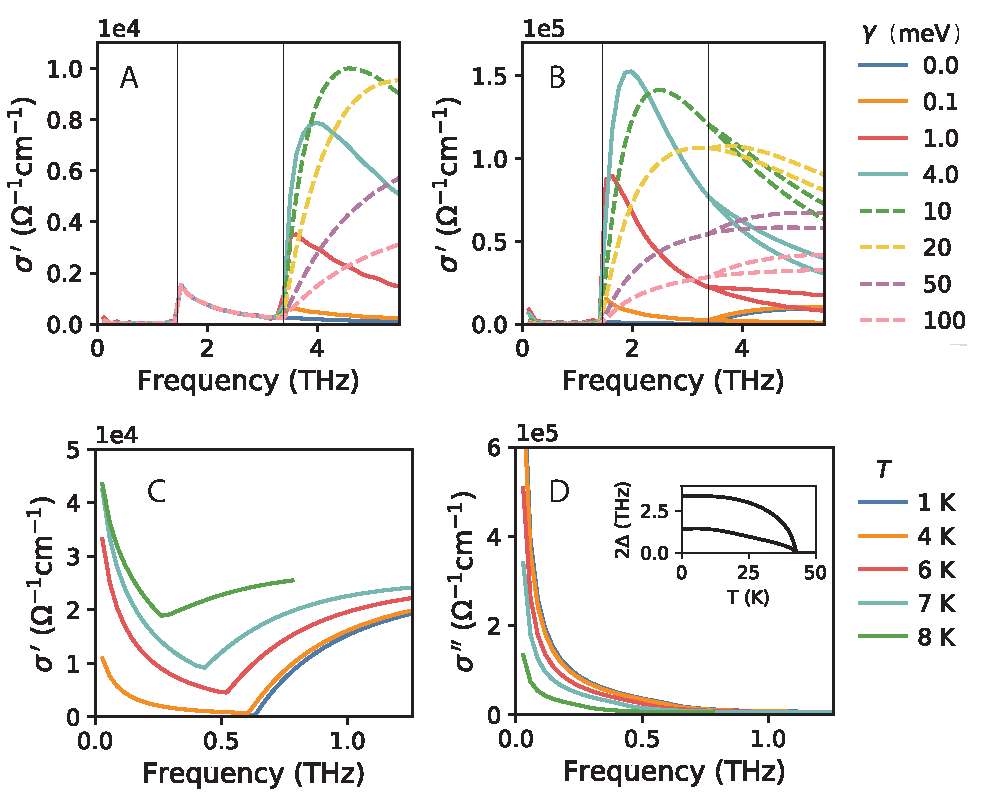
\includegraphics[width=\columnwidth]{figures/m-fig1.pdf}
	\caption{Real part $\sigma'$ (a,c) and imaginary part $\sigma''$ (b,d)
		of optical conductivities to first order in $A$ 
	for various impurity scattering rates at $T=\SI{4}{\kelvin}$ (A,B) and
various temperatures at $\gamma/2\Delta=10$. $\sigma'$ show a characteristic
conductivity gap below $T_C$ and both $\sigma'$, $\sigma''$ diverges as
$1/\omega$ in the static limit.}
\label{fig:cond-lin2}
\end{figure}
\begin{figure}[t]
  \centering
  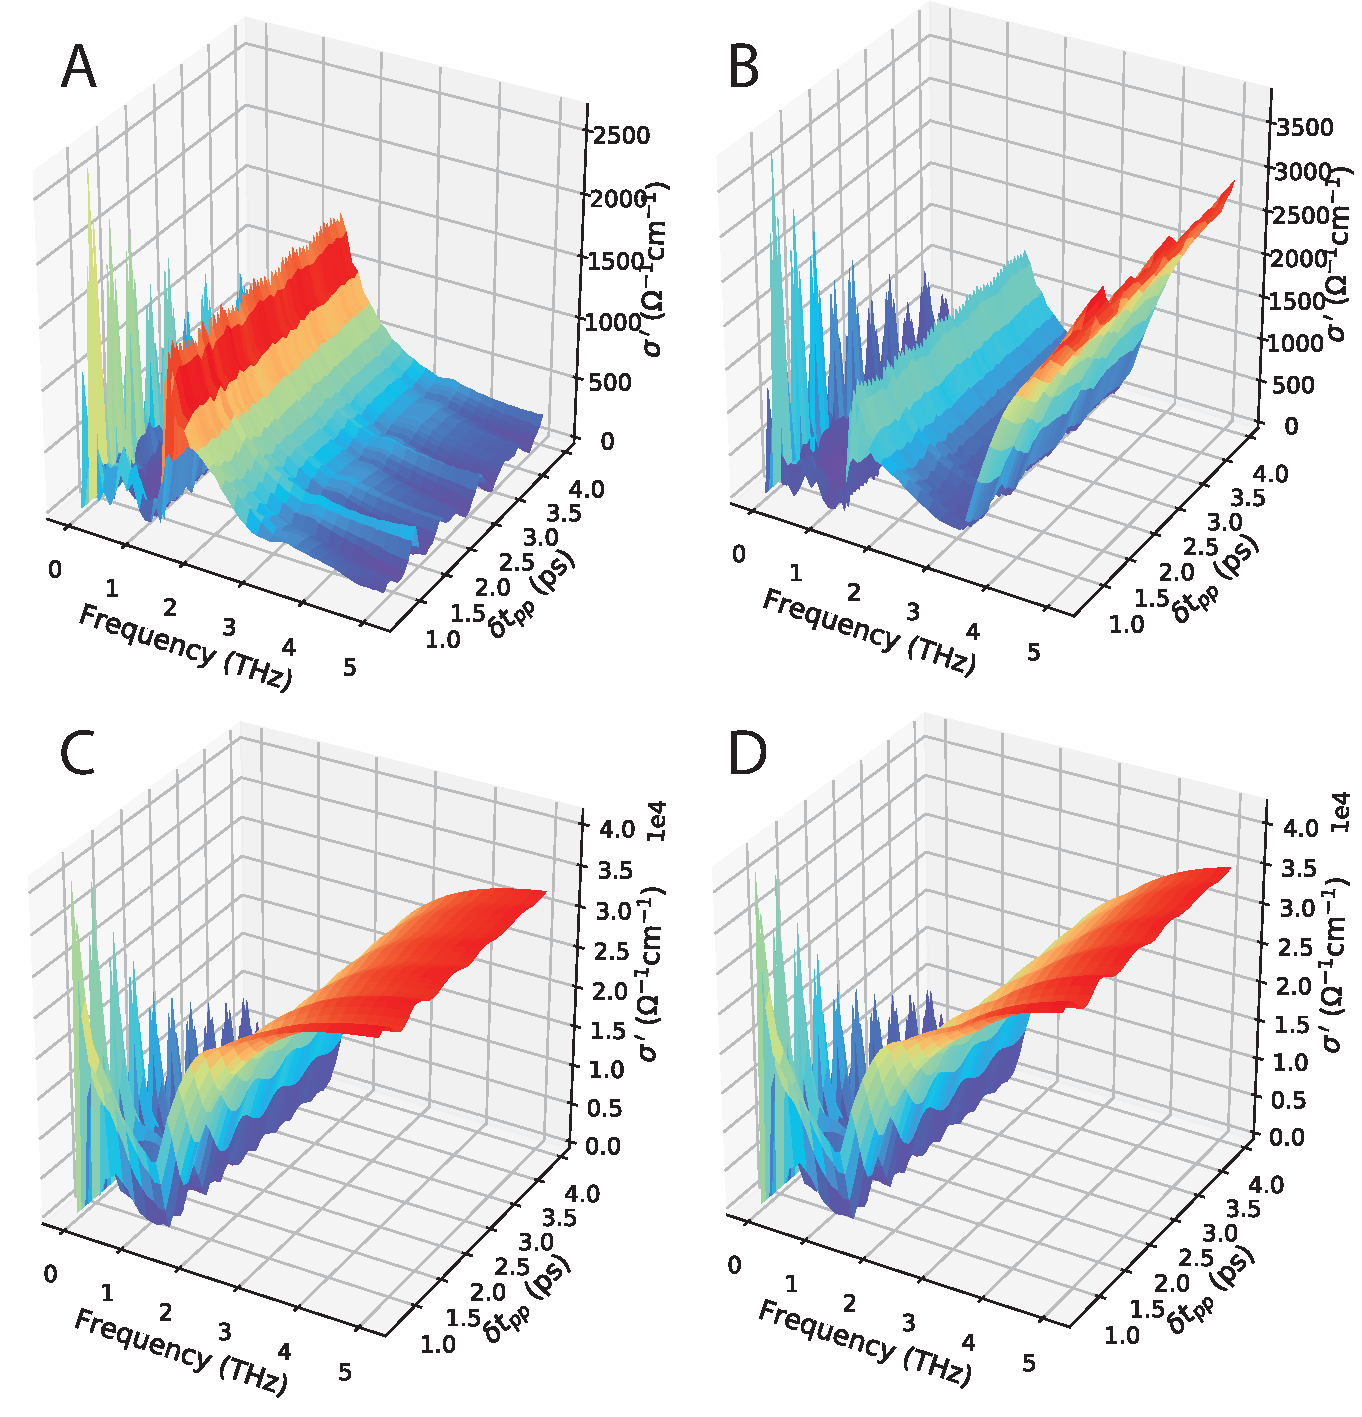
\includegraphics[width=\columnwidth]{figures/fig-cond-2d-fourcases}
  \caption{Time-resolved optical conductivity for the case were bands are in the
  limit (a) clean-clean, (b) clean-dirty, (c) dirty-clean, (d) dirty-dirty.}
\end{figure}

Motivation by the good agreement of the theory with experimental data, we now
discuss the case of a two-band superconductor. Here, the superconducting state
of MgB$_2$ is likely the most widely studied example and we adopt it as a
reference material. We loosely model the
$\pi$- and $\sigma$-bands believed to be responsible for superconductivity by
choosing material parameters 
$\Delta_{\pi}=\SI{3}{\milli\electronvolt}$,
$\Delta_{\sigma}=\SI{7}{\milli\electronvolt}$, 
$\varepsilon_{F,\pi}=\SI{2.9}{\electronvolt}$,
$\varepsilon_{F,\sigma}=\SI{0.7}{\electronvolt}$, 
$m_\pi=0.85m_e$,
$m_\sigma=1.38 m_e$, 
$\omega_D=\SI{50}{\milli\electronvolt}$,
$s_\pi=1$,
$s_\sigma=-1$.

\subsection{Optical conductivity}





\begin{figure*}[ht]
  \centering
  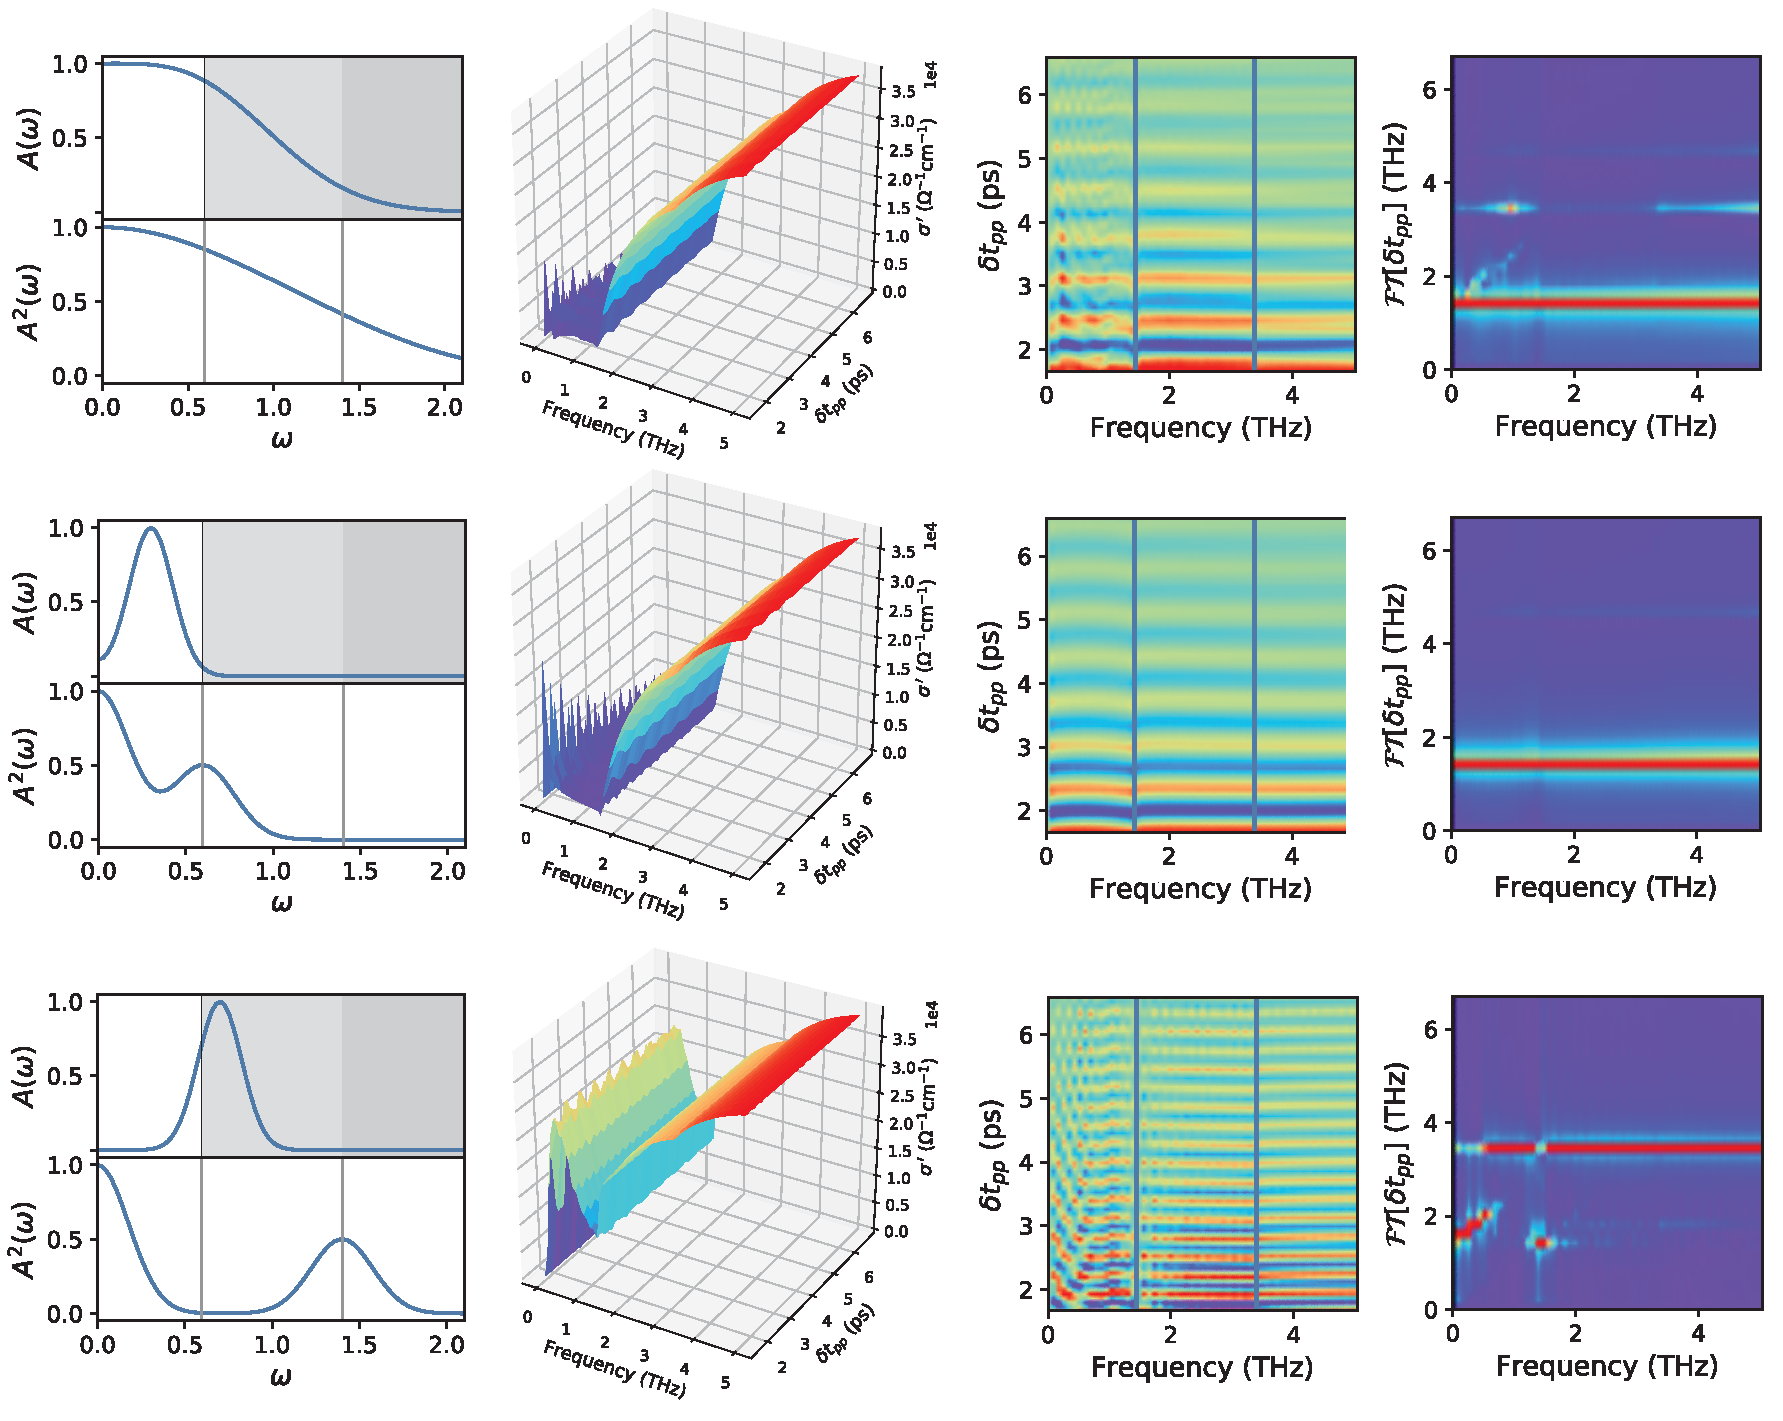
\includegraphics[width=\textwidth]{figures/fig-three-pulses}
  \caption{Time-resolved optical conductivity for three different pulses.}
\end{figure*}









%%%%%%%%%%%%%%%%%%%%%%%%%%%%%%%%%%%%%%%%%%%%%%%%%%%%%%%%
\subsection{Leggett mode and THG} 
\label{sec:leggett_mode}
%%%%%%%%%%%%%%%%%%%%%%%%%%%%%%%%%%%%%%%%%%%%%%%%%%%%%%%%

\begin{figure}[ht]
  \centering
  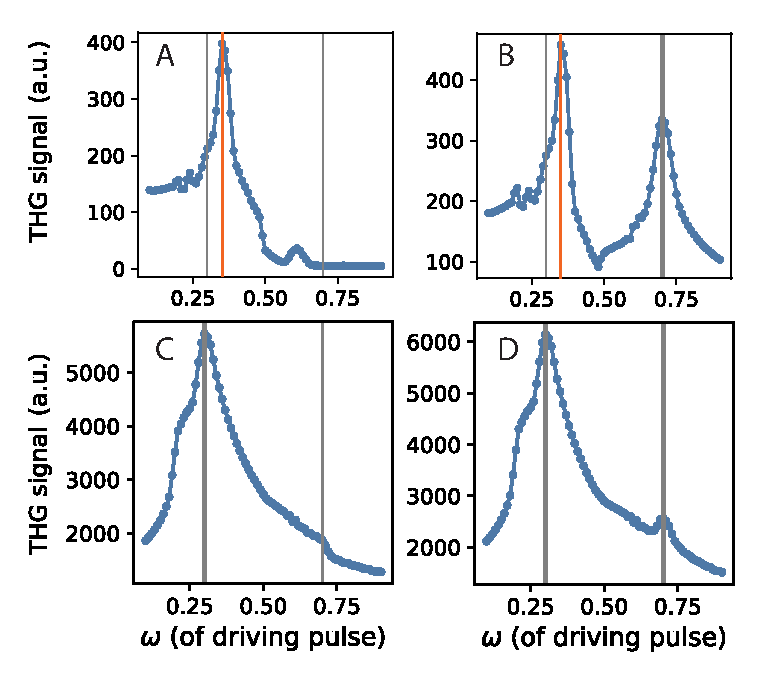
\includegraphics[width=\columnwidth]{figures/fig-driving}
  \caption{Caption}
\end{figure}
\begin{figure}[ht]
  \centering
  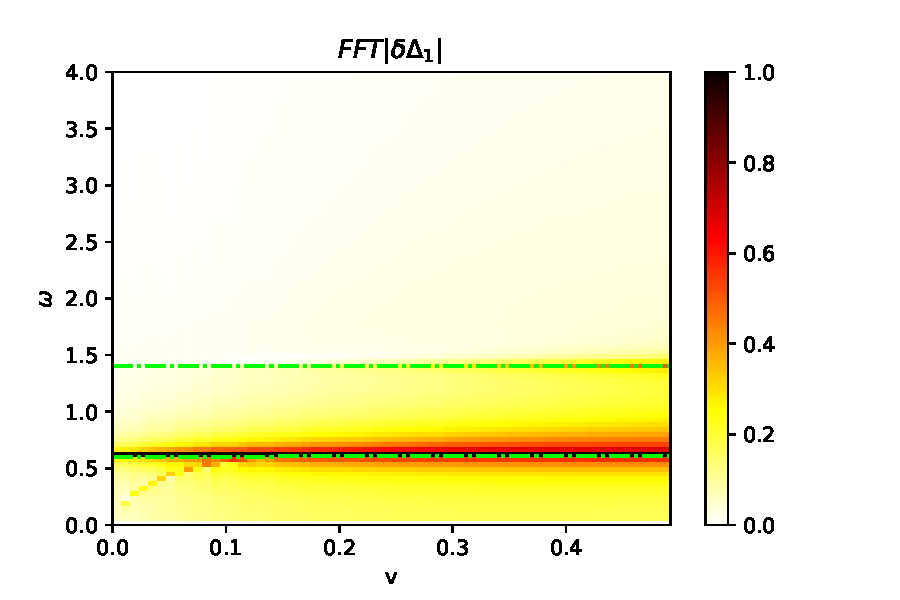
\includegraphics[width=\columnwidth]{figures/2_a}
  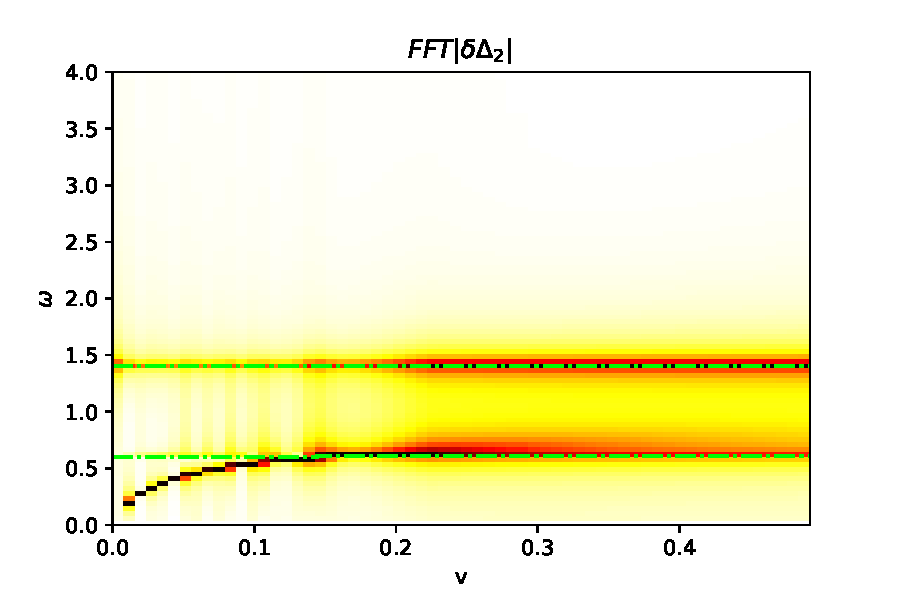
\includegraphics[width=\columnwidth]{figures/2_b}
\end{figure}

\begin{itemize}
	\item Definition, equation of Leggett mode
	\item Leggett equation of motion (equation for imaginary part of gap)
	  completely decouples from the remaining system of equations!
	\item In light of this - does Leggett mode really couple with Higgs
	  mode? Here the issue of the Fourier-transform comes up again. Is it
	  possible that the Fourier-transform of the whole time-range is the
	  correct approach. A point is that Leggett mode is peaked in between
	  the two gaps, but all oscillation contirbutions above $2\Delta_1$ are
	  damped very fast (exponential) so that at later times it looks like
	  the energy of the mode is $2\Delta_1$.
	\item TGH experiment. Here, let's decompose the THG signal in
	  quasiparticle, Higgs, Leggett contributions and show the THG in two
	  ways. First, a plot as a function of frequency for the four impurity
	  cases. Second, a plot as a function of temperature for the four cases.
	  The two plots should agree qualitatively, since changing the
	  temperature changes the gap (this is what experimentalists do).
	  Additionally, however, thermal effects contribute which might make
	  things a bit harder to see.
\end{itemize}


\begin{itemize}
	\item Discuss Fig. 5 for varying coupling strength and compare with clean limit result
\end{itemize}

Leggett mode has been potentially measured in between the two gaps. Discuss this
and also refer to Schnyder Nature Comm. 
 

%%%%%%%%%%%%%%%%%%%%%%%%%%%%%%%%%%%%%%%%%%%%%%%%%%%%%%%%
\section{Conclusion}
\label{sec:conclusion}
%%%%%%%%%%%%%%%%%%%%%%%%%%%%%%%%%%%%%%%%%%%%%%%%%%%%%%%%

...







%%%%%%%%%%%%%%%%%%%%%%%%%%%%%%%%%%%%%%%%%%%%%%%%%%%%%%%%
\begin{acknowledgments}
...
\end{acknowledgments}
%%%%%%%%%%%%%%%%%%%%%%%%%%%%%%%%%%%%%%%%%%%%%%%%%%%%%%%%






%%%%%%%%%%%%%%%%%%%%%%%%%%%%%%%%%%%%%%%%%%%%%%%%%%%%%%%%
\bibliography{literature}
%%%%%%%%%%%%%%%%%%%%%%%%%%%%%%%%%%%%%%%%%%%%%%%%%%%%%%%%




%%%%%%%%%%%%%%%%%%%%%%%%%%%%%%%%%%%%%%%%%%%%%%%%%%%%%%%%
%\end{comment}
\newpage
\appendix
%%%%%%%%%%%%%%%%%%%%%%%%%%%%%%%%%%%%%%%%%%%%%%%%%%%%%%%%
\section{Mattis-Bardeen substitution}
\label{apdx:MB}

One starts with the following assumption:

\begin{eqnarray*}
	\rho_k(R) = \langle \phi_\mathbf{k}^*(\mathbf{r})
	\phi_\mathbf{k}(\mathbf{r}') \rangle_{Av}
	=
	\frac{\sin k R}{k R} e^{-R/2l}
\end{eqnarray*}
where $R=\left|\mathbf{r}-\mathbf{r}'\right|$ and $\langle \, \rangle_{Av} =
\int_{}^{}\frac{d\Omega_\mathbf{k}}{4\pi}(\,)$ denotes
averaging over the angle of $\mathbf{k}$. $l$ is the mean-free path.
\begin{eqnarray*}
	&&\langle 
	\left|J^i_{\mathbf{k}\mathbf{k}'}\right|^2 
	\rangle_{Av}
	\\
	&=&
	\frac{e^2}{m^2} 
	\left|
	\int_{}^{} d^3\mathbf{r} \phi_\mathbf{k}^*(\mathbf{r})
	\frac{\partial_i}{i} \phi_{\mathbf{k}'}(\mathbf{r})
	\right|^2
	\\
	&=& \frac{e^2}{m^2} 
	\int_{}^{}\int_{}^{}\frac{d\Omega_\mathbf{k}}{4\pi}
	\frac{d\Omega_{\mathbf{k}'}}{4\pi}
		\int_{}^{} d^3\mathbf{r} \phi_\mathbf{k}^*(\mathbf{r})
		\frac{\partial_i}{i} \phi_{\mathbf{k}'}(\mathbf{r})
		\int_{}^{} d^3\mathbf{r}' \phi_\mathbf{k}(\mathbf{r}')
		 \frac{\partial_i'}{i} \phi_{\mathbf{k}'}^*(\mathbf{r'})
	\\
	&=& \frac{e^2}{m^2} 
	\int_{}^{}\int_{}^{}
	\frac{d\Omega_\mathbf{k}}{4\pi}
	\frac{d\Omega_{\mathbf{k}'}}{4\pi}
		\int_{}^{} d^3\mathbf{r} 
		\phi_\mathbf{k}^*(\mathbf{r})
		\frac{\partial_i}{i} \phi_{\mathbf{k}'}(\mathbf{r})
		\int_{}^{} d^3\mathbf{r}' 
		\left(-\frac{\partial_i'}{i}\phi_\mathbf{k}(\mathbf{r}')\right)
		\phi_{\mathbf{k}'}^*(\mathbf{r'})
	\\
	&=& \frac{e^2}{m^2} 
		\int_{}^{} d^3\mathbf{r} 
		d^3\mathbf{r}' 
	\int_{}^{}
	\frac{d\Omega_\mathbf{k}}{4\pi}
		\phi_\mathbf{k}^*(\mathbf{r})
		\partial_i'\phi_\mathbf{k}(\mathbf{r}')
	\int_{}^{}
	\frac{d\Omega_{\mathbf{k}'}}{4\pi}
		\phi_{\mathbf{k}'}^*(\mathbf{r'})
		\partial_i \phi_{\mathbf{k}'}(\mathbf{r})
	\\
	&=& \frac{e^2}{m^2} 
		\int_{}^{} d^3\mathbf{r} 
		d^3\mathbf{r}' 
		\partial_i'
		\langle 
		\phi_\mathbf{k}^*(\mathbf{r})
		\phi_\mathbf{k}(\mathbf{r}')
		\rangle_{Av}
		\partial_i 
		\langle 
		\phi_{\mathbf{k}'}^*(\mathbf{r'})
		\phi_{\mathbf{k}'}(\mathbf{r})
		\rangle_{Av}
	\\
	&=& \frac{e^2}{m^2} V
		\int_{}^{} d^3\mathbf{R} 
		\frac{\partial \rho_k(R)}{\partial R_i}
		\frac{\partial \rho_{k'}(R)}{\partial R_i}
	\\
	&=& \frac{e^2}{m^2} V
		\int_{}^{} d^3\mathbf{R} 
		\frac{R_i^2}{R^2}
		\frac{\partial \rho_k(R)}{\partial R}
		\frac{\partial \rho_{k'}(R)}{\partial R}
	\\
	&\approx& \frac{e^2}{m^2} V
		\int_{}^{} d^3\mathbf{R} 
		\frac{R_i^2}{R^2}
		\frac{e^{-R/l}}{2R^2} \cos (k-k')R
	\\
	&=& \frac{e^2}{m^2} V
		\int_{0}^{\infty}dR
		\int_{0}^{2\pi}d\varphi
		\int_{0}^{\pi}d\theta
		R^2 \sin \theta	
		\frac{R_i^2}{R^2}
		\frac{e^{-R/l}}{2R^2} \cos (k-k')R
\end{eqnarray*}
Now we make use of the fact that
\begin{eqnarray*}
		\int_{0}^{2\pi}d\varphi
		\int_{0}^{\pi}d\theta
		\sin \theta	
		\frac{R_i^2}{R^2}
		= \frac{4\pi}{3}
\end{eqnarray*}
We see that the expression is now independent of the component index $i$ of the
real-space vector $\mathbf{J}_{\mathbf{k}\mathbf{k}'}$. This means that
averaging over angles in momentum space results in loss of polarization
dependence in real-space.

Performing the remaining integral gives 
\begin{eqnarray*}
	\langle 
	\left|J^i_{\mathbf{k}\mathbf{k}'}\right|^2 
	\rangle_{Av}
	&=& 
	\frac{2\pi}{3}\frac{e^2}{m^2} V
		\int_{0}^{\infty}dR
		e^{-R/l} \cos (k-k')R
	\\
	&=& 
	\frac{2\pi}{3}\frac{e^2}{m^2} V
	\frac{1/l}{(1/l)^2+ (k-k')^2}
\end{eqnarray*}
Close to the Fermi surface we have $\varepsilon_\mathbf{k}=v_F(k-k_F)$ which
yields
\begin{eqnarray*}
	\langle 
	\left|J^i_{\mathbf{k}\mathbf{k}'}\right|^2 
	\rangle_{Av}
	&=& 
	\frac{2\pi}{3}\frac{e^2}{m^2} V
	\frac{1/l}{(1/l)^2+ (\varepsilon_k-\varepsilon_{k'})^2/v_F^2}
\end{eqnarray*}

\section{Model}

\label{apdx:model}
\begin{eqnarray}
  \mathcal{H}_0 = \sum_{i\mathbf{k}\sigma}  
	\varepsilon_{i\mathbf{k}}c_{i\mathbf{k}\sigma}^\dagger
	c_{i\mathbf{k}\sigma} + \sum_{i\mathbf{k}}^{}
	\left( \Delta_i c_{i\mathbf{-k}\uparrow }^\dagger
	c_{i\mathbf{k}\downarrow }^\dagger  \right) \,,
\end{eqnarray}

where $\varepsilon_{i\mathbf{k}} = s_i \left(\mathbf{k}^2/2m_i -
\varepsilon_{F_i}\right)$ and the superconducting order parameter is self-consistently determined by 
$\Delta_i = \sum_{j\mathbf{k}}^{}U_{ij} \langle c_{j-\mathbf{k}\downarrow
}c_{j\mathbf{k}\uparrow }\rangle$.

\begin{eqnarray*}
	\mathcal{H}_1 = -\sum_{i\mathbf{kk'}\sigma}^{}
	\mathbf{J}_{i\mathbf{kk'}} \cdot \mathbf{A} \,
	c_{i\mathbf{k}\sigma}^\dagger  c_{i\mathbf{k}'\sigma} +
	\sum_{i\mathbf{k}\sigma}^{} \frac{s_i e^2}{2m_i} \mathbf{A}^2 \,
	c_{i\mathbf{k}\sigma}^\dagger c_{i\mathbf{k}\sigma}
\end{eqnarray*}

\begin{eqnarray*}
	\langle \left|\mathbf{e} \cdot
	\mathbf{J}_{i\mathbf{kk'}}\right|^2\rangle_{\text{Av}}
	&=& \int \frac{d\Omega_\mathbf{k}}{4\pi} \frac{d\Omega_\mathbf{k}'}{4\pi}
	\left|\mathbf{e} \cdot \mathbf{J}_{i\mathbf{kk'}}\right|^2
	\\
	&\approx& \frac{(e v_{F_i})^2}{3 \pi N_i(0)} 
	\frac{\gamma_i}{(\varepsilon-\varepsilon')^2 + \gamma_i^2}
\end{eqnarray*}

Discussion of $A, A^2$.

The full Hamiltonian is given by $\mathcal{H} = \mathcal{H}_0 +
\mathcal{H}_1$.

\begin{eqnarray*}
  \mathbf{j} = - \bigg\langle \frac{\delta\mathcal{H}}{\delta
  \mathbf{A}}\bigg\rangle = \mathbf{j}_P + \mathbf{j}_D
\end{eqnarray*}
\begin{eqnarray*}
  \mathbf{j}_P = \sum_{i\mathbf{kk'}\sigma}^{}
	\mathbf{J}_{i\mathbf{kk'}} \cdot \mathbf{A} \,
	\langle 
	c_{i\mathbf{k}\sigma}^\dagger  c_{i\mathbf{k}'\sigma}
	\rangle
\end{eqnarray*}
\begin{eqnarray*}
  \mathbf{j}_D = -\sum_{i\mathbf{k}\sigma}^{} \frac{s_i e^2}{2m_i} 
  \mathbf{A} \,
  \langle 
  c_{i\mathbf{k}\sigma}^\dagger c_{i\mathbf{k}\sigma}
  \rangle
\end{eqnarray*}

Next we construct the density matrix
\begin{eqnarray*}
  \rho = \ket{\psi_0}\bra{\psi_0} = 
  \begin{pmatrix}
    \rho_{i\mathbf{kk'}}^{11} &
    \rho_{i\mathbf{kk'}}^{12} \\
    \rho_{i\mathbf{kk'}}^{21} &
    \rho_{i\mathbf{kk'}}^{22}
  \end{pmatrix}
  =
  \begin{pmatrix}
    \langle c_{i\mathbf{k}\uparrow }^\dagger c_{i\mathbf{k}'\uparrow }\rangle
    &
    \langle c_{i\mathbf{k}\uparrow }^\dagger c_{i-\mathbf{k}'\downarrow
    }^\dagger \rangle
    \\
    \langle 
    c_{i-\mathbf{k}\downarrow }c_{i\mathbf{k'}\uparrow }
    \rangle
    &
    \langle 
    c_{i-\mathbf{k}\downarrow }c_{i\mathbf{-k'}\downarrow }^\dagger 
    \rangle
  \end{pmatrix}
\end{eqnarray*}
Writing the density matrix in vector form,
\begin{eqnarray*}
  \rho = 
  \begin{pmatrix}
    \rho_{i\mathbf{kk'}}^{11} \\
    \rho_{i\mathbf{kk'}}^{12} \\
    \rho_{i\mathbf{kk'}}^{21} \\
    \rho_{i\mathbf{kk'}}^{22}
  \end{pmatrix} \,,
\end{eqnarray*}
the Heisenberg equation of motion can be calculated as follows
\begin{eqnarray*}
  i\frac{d \rho_{i\mathbf{k}\mathbf{k}'}}{dt}
  =
  \sum_{\mathbf{q}}^{}
  \left[ 
    H_{i\mathbf{k}' \mathbf{q}}^{(1)} \rho_{i\mathbf{kq}} -
    H_{i\mathbf{qk}}^{(2)}
    \rho_{i\mathbf{qk'}}
  \right]
\end{eqnarray*}
where we have defined the following two matrices:
\begin{eqnarray*}
  H_{i\mathbf{kk'}}^{(1)}
  =
  \begin{pmatrix}
    h_{i\mathbf{kk'}}^{11} & h_{i\mathbf{kk'}}^{12} & & \\
    h_{i\mathbf{kk'}}^{21} & h_{i\mathbf{kk'}}^{22} & & \\
    && h_{i\mathbf{kk'}}^{11} & h_{i\mathbf{kk'}}^{12} \\
    && h_{i\mathbf{kk'}}^{21} & h_{i\mathbf{kk'}}^{22} & 
  \end{pmatrix}
\end{eqnarray*}
\begin{eqnarray*}
  H_{i\mathbf{kk'}}^{(2)}
  =
  \begin{pmatrix}
    h_{i\mathbf{kk'}}^{11} && h_{i\mathbf{kk'}}^{21} & \\
    & h_{i\mathbf{kk'}}^{11} && h_{i\mathbf{kk'}}^{21} \\
    h_{i\mathbf{kk'}}^{12} && h_{i\mathbf{kk'}}^{22} & \\
    & h_{i\mathbf{kk'}}^{12} && h_{i\mathbf{kk'}}^{22}
  \end{pmatrix}
\end{eqnarray*}
\begin{comment}
Let us multiply this out:
\begin{eqnarray*}
  i \frac{d}{dt}
  \begin{pmatrix}
    \rho_{i\mathbf{kk'}}^{11} &
    \rho_{i\mathbf{kk'}}^{12} \\
    \rho_{i\mathbf{kk'}}^{21} &
    \rho_{i\mathbf{kk'}}^{22}
  \end{pmatrix}
  =
  \sum_{\mathbf{q}}^{}
  \begin{pmatrix}
    h_{i\mathbf{k'q}}^{11} \rho_{i\mathbf{kq}}^{11}
    + h_{i\mathbf{k'q}}^{12} \rho_{i\mathbf{kq}}^{12}
    -h_{i\mathbf{qk}}^{11} \rho_{i\mathbf{qk'}}^{11}
    -h_{i\mathbf{qk}}^{21} \rho_{i\mathbf{qk'}}^{21}
    &
    h_{i\mathbf{k'q}}^{21} \rho_{i\mathbf{kq}}^{11}
    + h_{i\mathbf{k'q}}^{22} \rho_{i\mathbf{kq}}^{12}
    -h_{i\mathbf{qk}}^{11} \rho_{i\mathbf{qk'}}^{12}
    -h_{i\mathbf{qk}}^{21} \rho_{i\mathbf{qk'}}^{22}
    \\
    h_{i\mathbf{k'q}}^{11} \rho_{i\mathbf{kq}}^{21}
    + h_{i\mathbf{k'q}}^{12} \rho_{i\mathbf{kq}}^{22}
    -h_{i\mathbf{qk}}^{12} \rho_{i\mathbf{qk'}}^{11}
    -h_{i\mathbf{qk}}^{22} \rho_{i\mathbf{qk'}}^{21}
    &
    h_{i\mathbf{k'q}}^{21} \rho_{i\mathbf{kq}}^{21}
    + h_{i\mathbf{k'q}}^{22} \rho_{i\mathbf{kq}}^{22}
    -h_{i\mathbf{qk}}^{12} \rho_{i\mathbf{qk'}}^{12}
    -h_{i\mathbf{qk}}^{22} \rho_{i\mathbf{qk'}}^{22}
  \end{pmatrix}
\end{eqnarray*}
\end{comment}

Now we expand the equation of motion in orders of $\mathbf{A}$. The zeroth-order
components are:
\begin{eqnarray*}
  \rho_{i\mathbf{kk'}}\big|_0 = \delta_{kk'} 
  \begin{pmatrix}
    \frac{1}{2}\left(1-\frac{\varepsilon_{i\mathbf{k}}}{E_{i\mathbf{k}}}\right)
    +\frac{\varepsilon_{i\mathbf{k}}}{ E_{i\mathbf{k}}}f_{i\mathbf{k}}
    \\
    -\frac{\Delta^{eq}_i}{2}(1-2f_{i\mathbf{k}})
    \\
    -\frac{\Delta^{eq}_i}{2}(1-2f_{i\mathbf{k}})
    \\
    \frac{1}{2}\left(1+\frac{\varepsilon_{i\mathbf{k}}}{E_{i\mathbf{k}}}\right)
    -\frac{\varepsilon_{i\mathbf{k}}}{ E_{i\mathbf{k}}}f_{i\mathbf{k}}
  \end{pmatrix}
\end{eqnarray*}
\begin{eqnarray*}
  H_{i\mathbf{kk'}}^{(1)}\big|_0
  =
  \delta_{\mathbf{kk'}}
  \begin{pmatrix}
    \varepsilon_{i\mathbf{k}} & \Delta^{eq}_i & & \\
    \Delta^{eq}_i & -\varepsilon_{i\mathbf{k}} & & \\
    && \varepsilon_{i\mathbf{k}} & \Delta^{eq}_i \\
    && \Delta^{eq}_i & -\varepsilon_{i\mathbf{k}} & 
  \end{pmatrix}
\end{eqnarray*}
\begin{eqnarray*}
  H_{i\mathbf{kk'}}^{(2)}\big|_0
  =
  \delta_{\mathbf{kk'}}
  \begin{pmatrix}
    \varepsilon_{i\mathbf{k}} && \Delta^{eq}_i & \\
    & \varepsilon_{i\mathbf{k}} && \Delta^{eq}_i \\
    \Delta^{eq}_i && -\varepsilon_{i\mathbf{k}} & \\
    & \Delta^{eq}_i && -\varepsilon_{i\mathbf{k}}
  \end{pmatrix}
\end{eqnarray*}

Now we proceed with the first order.

\begin{eqnarray*}
i\frac{d}{dt} \rho_{i\mathbf{k}\mathbf{k}'}\big|_1
  &=&
  \left( 
    H_{i\mathbf{k}' \mathbf{k'}}^{(1)} 
    -
    H_{i\mathbf{kk}}^{(2)}
  \right)\bigg|_0
    \rho_{i\mathbf{kk'}}\big|_1
    \\
  &+&
  \left(
    H_{i\mathbf{k}' \mathbf{k}}^{(1)}\big|_1 \rho_{i\mathbf{kk}}\big|_0 
    -
    H_{i\mathbf{k'k}}^{(2)}\big|_1
    \rho_{i\mathbf{k'k'}}\big|_0
  \right)
\end{eqnarray*}
\begin{eqnarray*}
  H_{i\mathbf{kk'}}^{(1)}\big|_0
  =
  -\mathbf{J}_{i\mathbf{kk'}} \cdot \mathbf{A} \,
  \begin{pmatrix}
    1 &  & & \\
     & -1 & & \\
    && 1 &  \\
    &&  & -1& 
  \end{pmatrix}
\end{eqnarray*}
\begin{eqnarray*}
  H_{i\mathbf{kk'}}^{(2)}\big|_0
  =
  -\mathbf{J}_{i\mathbf{kk'}} \cdot \mathbf{A} \,
  \begin{pmatrix}
    1 &&  & \\
    & 1 &&  \\
     && -1 & \\
    &  &&-1 
  \end{pmatrix}
\end{eqnarray*}

The second order is

\begin{eqnarray*}
  i\frac{d \rho_{i\mathbf{k}\mathbf{k}}}{dt}
  &=&
    \left( 
      H_{i\mathbf{kk}}^{(1)}  - H_{i\mathbf{kk}}^{(2)} 
    \right)\bigg|_0
    \rho_{i\mathbf{kk}}\big|_2
    \\
    &+&
    \sum_{\mathbf{q}}^{}
    \left( 
    H_{i\mathbf{kq}}^{(1)}\big|_1 \rho_{i\mathbf{kq}}\big|_1 -
    H_{i\mathbf{qk}}^{(2)}\big|_1 \rho_{i\mathbf{qk}}\big|_1
    \right)
    \\
    &+&
    \left( 
      H_{i\mathbf{kk}}^{(1)} - H_{i\mathbf{kk}}^{(2)} 
    \right)\bigg|_2
      \rho_{i\mathbf{kk}}\big|_0
\end{eqnarray*}
\begin{eqnarray*}
  H_{i\mathbf{kk}}^{(1,2)}\big|_2 = 
  H_{i\mathbf{kk}}^{(1,2)}\big|_{2,D}
  +H_{i\mathbf{kk}}^{(1,2)}\big|_{2,H}
  +H_{i\mathbf{kk}}^{(1,2)}\big|_{2,L}
\end{eqnarray*}
Diamagnetic quasiparticle current contribution
\begin{eqnarray*}
  H_{i\mathbf{kk'}}^{(1)}\big|_{0,D}
  =
  \delta_{\mathbf{kk'}} \frac{s_ie^2}{2m_i}\mathbf{A}^2
  \begin{pmatrix}
    1 &  & & \\
     & -1 & & \\
    && 1 &  \\
    &&  & -1& 
  \end{pmatrix}
\end{eqnarray*}
\begin{eqnarray*}
  H_{i\mathbf{kk'}}^{(2)}\big|_{0,D}
  =
  \delta_{\mathbf{kk'}} \frac{s_ie^2}{2m_i}\mathbf{A}^2
  \begin{pmatrix}
    1 &&  & \\
    & 1 &&  \\
     && -1 & \\
    &  &&-1 
  \end{pmatrix}
\end{eqnarray*}
Higgs contribution
\begin{eqnarray*}
  H_{i\mathbf{kk'}}^{(1)}\big|_{0,D}
  =
  \delta_{\mathbf{kk'}} \delta \Delta'\big|_2
  \begin{pmatrix}
     & 1 & & \\
    1 &  & & \\
    &&  & 1 \\
    && 1 &  & 
  \end{pmatrix}
\end{eqnarray*}
\begin{eqnarray*}
  H_{i\mathbf{kk'}}^{(2)}\big|_{0,D}
  =
  \delta_{\mathbf{kk'}} \delta \Delta'\big|_2
  \begin{pmatrix}
     && 1 & \\
    &  && 1 \\
    1 &&  & \\
    & 1 && 
  \end{pmatrix}
\end{eqnarray*}
Leggett contribution
\begin{eqnarray*}
  H_{i\mathbf{kk'}}^{(1)}\big|_{0,D}
  =
  \delta_{\mathbf{kk'}} \delta \Delta''\big|_2
  \begin{pmatrix}
     & i & & \\
    -i &  & & \\
    &&  & i \\
    && -i &  & 
  \end{pmatrix}
\end{eqnarray*}
\begin{eqnarray*}
  H_{i\mathbf{kk'}}^{(2)}\big|_{0,D}
  =
  \delta_{\mathbf{kk'}} \delta \Delta''\big|_2
  \begin{pmatrix}
     && -i & \\
    &  && -i \\
    i &&  & \\
    & i && 
  \end{pmatrix}
\end{eqnarray*}

And third order
\begin{eqnarray*}
i\frac{d}{dt} \rho_{i\mathbf{k}\mathbf{k}'}\big|_3
  &=&
  \left( 
    H_{i\mathbf{k'k'}}^{(1)} - H_{i\mathbf{kk} }^{(2)} 
  \right)\bigg|_0
    \rho_{i\mathbf{kk'}}\big|_3
    \\
	&+&
  \sum_{\mathbf{q}}^{}
  \left( 
    H_{i\mathbf{k'q}}^{(1)}\big|_1 \rho_{i\mathbf{kq }}\big|_2 -
    H_{i\mathbf{qk} }^{(2)}\big|_1 \rho_{i\mathbf{qk'}}\big|_2
  \right)
  \\
	&+&
  \left( 
    H_{i\mathbf{k'k'}}^{(1)} - H_{i\mathbf{kk} }^{(2)} 
  \right)\bigg|_2
    \rho_{i\mathbf{kk'}}\big|_1
\end{eqnarray*}

\end{document}
 
 
\begin{eqnarray*}
  H_{i\mathbf{kk'}}^{(1)}\big|_{0,D}
  =
  \begin{pmatrix}
    h11 & h12 & & \\
    h21 & h22 & & \\
    && h11 & h12 \\
    && h21 & h22 & 
  \end{pmatrix}
\end{eqnarray*}
\begin{eqnarray*}
  H_{i\mathbf{kk'}}^{(2)}\big|_{0,D}
  =
  \begin{pmatrix}
    h11 && h21 & \\
    & h11 && h21 \\
    h12 && h22 & \\
    & h12 && h22
  \end{pmatrix}
\end{eqnarray*}
%%%%%%%%%%%%%%%%%%%%%%%%%%%%%%%%%%%%%%%%%%%%%%%%%%%%%%%%
\section{Derivation of nonequilibrium optical conductivity}
\label{sec:derivation_noneq_cond}
%%%%%%%%%%%%%%%%%%%%%%%%%%%%%%%%%%%%%%%%%%%%%%%%%%%%%%%%


\begin{itemize}
	\item Put here all equations and derivations of the main results
\end{itemize}






%%%%%%%%%%%%%%%%%%%%%%%%%%%%%%%%%%%%%%%%%%%%%%%%%%%%%%%%
\section{Influence of pump pulse frequency}
\label{sec:influence_pump_pulse_freq}
%%%%%%%%%%%%%%%%%%%%%%%%%%%%%%%%%%%%%%%%%%%%%%%%%%%%%%%%

\begin{itemize}
	\item Discuss influence of pump pulse frequency and bandwith to excite only one or both Higgs mode
	\item Show result in Fig. 7
\end{itemize}


\end{document}
